\documentclass[]{beamer}
%Beamer Stuff
\usetheme{boxes}
\useoutertheme{infolines}
\setbeamercovered{invisible}
%Language
\usepackage[german]{babel}
\usepackage[utf8]{inputenc}
\usepackage[T1]{fontenc}
%Math
\usepackage{amsmath}
\usepackage{amsfonts}
\usepackage{amssymb}
\usepackage{amstext}
\usepackage{array}
%Environments

%Div
\setcounter{tocdepth}{2}
\DeclareMathOperator{\ggt}{ggT}
\DeclareMathOperator{\modm}{mod}
\DeclareMathOperator{\logl}{Log}
\renewcommand{\tt}{\overline}
\usepackage{enumerate}
%------------------------------
\begin{document}
\title{$B^{+}$-Bäume}
\subtitle{Algorithmen und Datenstrukturen II}
\author{Furch, Gabler, Herpers, Schmid}
\institute[HM]{Hochschule München}
\date{18. Juni 2018}

\begin{frame}[plain]
\titlepage
\end{frame}

\begin{frame}{$B^{+}$-Bäume}
$B^{+}$-Bäume mit Ordnung $m$ sind Indexbäume mit den folgenden Eigenschaften:
\begin{itemize}
	\item Alle Blätter haben die gleiche Tiefe.
	\item Jeder Knoten mit Ausnahme der Wurzel und der Blätter hat wenigstens m Kinder.
	\item Die Wurzel hat wenigstens 2 Kinder.
	\item Jeder Knoten hat höchstens $2m$ Kinder.
	\item Jeder Knoten mit $i$ Kindern hat $i-1$ Schlüssel.
\end{itemize}
\end{frame}

\begin{frame}{Search I}
\begin{itemize}
	\item Starte bei Wurzel
	\item Vergleiche ges. Schlüssel mit Schlüssel in Knoten und steige Ebene tiefer bis Knoten gefunden oder bei Blättern angekommen.
\end{itemize}
\end{frame}

\begin{frame}{Search II}
\begin{center}
	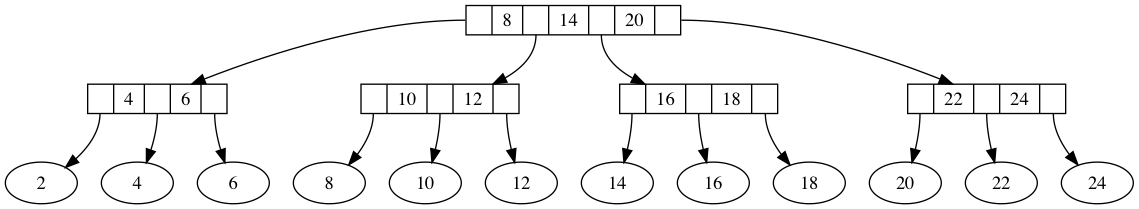
\includegraphics[scale=0.3]{example_11.png} \hspace{0.3cm}
\end{center}
\end{frame}

\begin{frame}{Insert I}
Einfügen eines Wertes $\omega$
\begin{itemize}
	\item Mit Search entsprechende Blattseite suchen.
	\item Passender Knoten $n<2m$ Elemente $\rightarrow$ $\omega$ einfügen
	\item Passender Knoten $n=2m$ Elemente $\rightarrow$ neuer Knoten erzeugen
	\begin{itemize}
		\item Die ersten $m$ Werte auf Originalknoten
		\item Die letzten $m$ Werte auf neuen Knoten
		\item Mittleres Element auf entsprechenden Knoten nach oben
		\item Vorgang rekursiv bis zur Wurzel wiederholen
	\end{itemize}
\end{itemize}
\end{frame}

\begin{frame}{Insert II}
\begin{center}
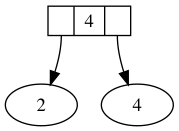
\includegraphics[scale=0.3]{example_1.png} \hspace{0.3cm}
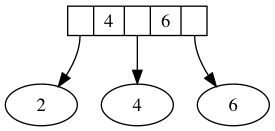
\includegraphics[scale=0.3]{example_2.png} \hspace{0.3cm}
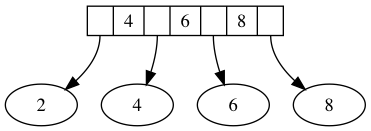
\includegraphics[scale=0.3]{example_3.png} \hspace{0.3cm}

\vspace{1cm}
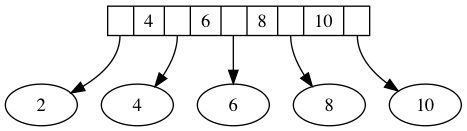
\includegraphics[scale=0.3]{example_4.png} \hspace{0.3cm}
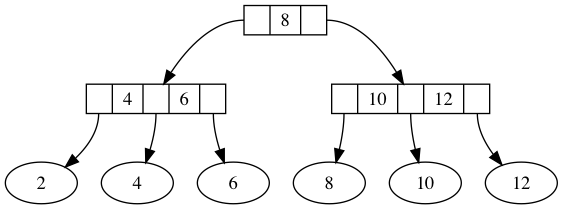
\includegraphics[scale=0.3]{example_5.png} \hspace{0.3cm}
\end{center}
\end{frame}

\begin{frame}{Insert III}
Insert 36

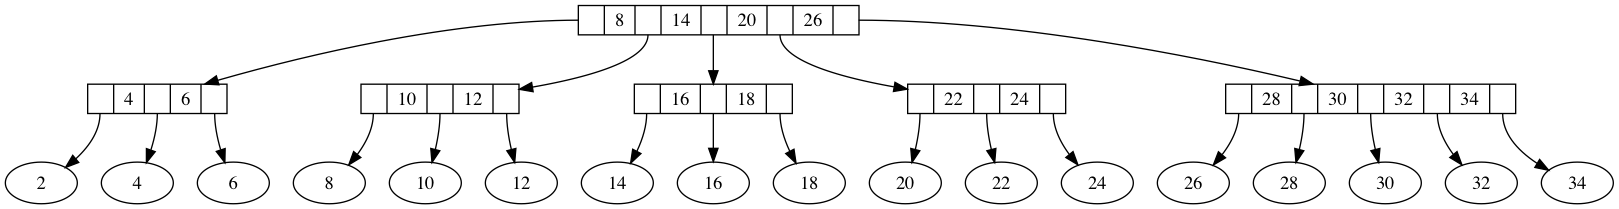
\includegraphics[width=\textwidth]{example_16.png}

\vspace{1cm}
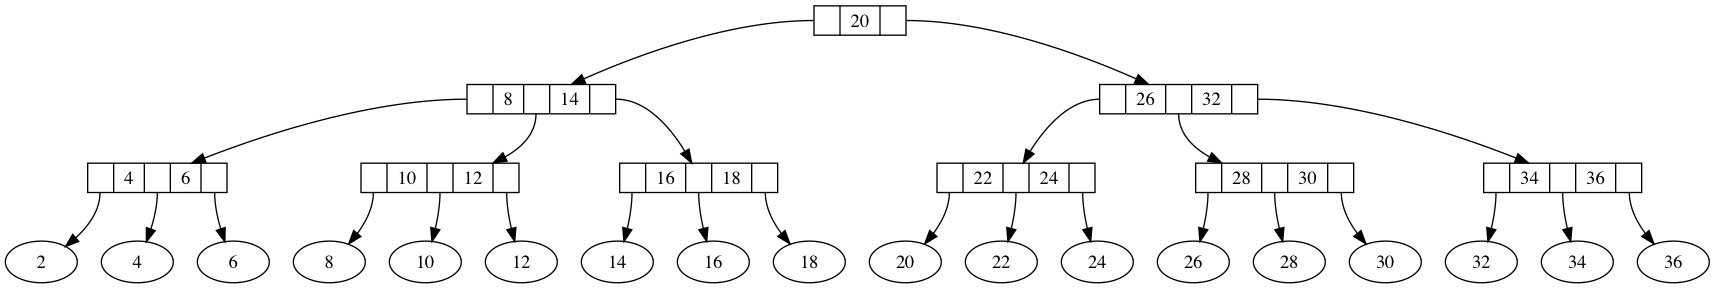
\includegraphics[width=\textwidth]{example_17.png}
\end{frame}

\begin{frame}{Remove I}
Löschen eines Wertes $\omega$
\begin{itemize}
	\item Mit Search entsprechende Stelle finden
	\item Falls $\omega$ auf Blattseite gespeichert $\rightarrow$ Wert löschen, evtl. Unterlauf behandeln
	\item Falls $\omega$ nicht auf Blattseite gespeichert $\rightarrow$ Wert durch nächst-kleineres Element ersetzen, evtl. Unterlauf behandeln
\end{itemize}
\end{frame}

\begin{frame}{Remove II}
Remove 8
\begin{center}
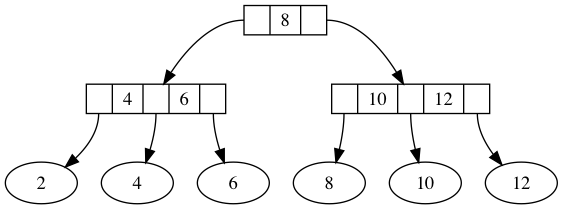
\includegraphics[scale=0.4]{example_5.png}

\vspace{1cm}
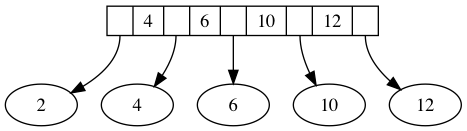
\includegraphics[scale=0.5]{example_6_rem.png}
\end{center}
\end{frame}

\end{document}